\chapter{Introduction} \label{ch:intro}

Generating an accurate and high precision model of its surrounding 
environment to indicate hazard features is an important issue for any 
autonomous vehicle. Knowing its own location in the map is essential for 
the vehicle to navigate and avoid obstacle autonomously. 

In many applications, the mobile robot has a priori map. The given 
priori map may be sufficient for localization purpose, but generally do 
not have the resolution required for obstacle detection. Ground vehicles 
need to deal with temporary added road block and parked cars. Aerial 
vehicles may not have a high enough resolution map that indicates tall 
trees, steep hills or electrical towers. In addition, usable map do not 
always exist. Without maps or externally referenced pose information, 
the robot must produce its own map and concurrently localize itself 
within the map. This problem is referred to as the simultaneous 
localization and mapping (SLAM). 

Traditional 2D SLAM algorithms are well established in the past
decade. A SLAM algorithm typically utilises measurements from several
types of sensor which can be divided into two groups, those that
provide vehicles pose and orientation measurements, such as wheel
odometry, or GPS; and those that provide landmark bearing and range
measurements, such as radar, sonar, laser range finder. In recent
years, optical sensors are actively being incorporated into SLAM
algorithm and successfully used in ground vehicle navigation. For
aerial vehicles, the experiments are mostly limited to simulation, and
results from realistic aerial video data is rare \ref{nemra_robust_2010}
\ref{jianli_unscented_2011} \ref{sunderhauf_using_2007} \ref{artieda_visual_2009}.

\section{Problem Statement}\label{section:ProblemStatement}
Obstacle detection has received a lot of research interest in recent 
years. Various algorithms were developed for ground, under water and 
aerial vehicle using different sensor such as sonar, radar, LIDAR, and 
vision. Most research focus on utilizing with only one sensor. Yet, 
research shows that using multiple sensors produces a better measurement 
than single sensor [reference in proposal]. With various sensors 
readily available on most UAV navigation hardware; such as 
accelerometers, gyroscope, GPS receiver, altimeter, etc., fully 
utilizing these sensors to aid the main OD sensor helps to improve the 
accuracy and robustness of the range measurement, especially in harsh 
flying condition. 

This thesis focuses on developing an obstacle detection system by using
a SLAM algorithm as a sensor fusion framework for medium size UAV
conduction low altitude terrain following flight in natural
environment.The obstacles are static objects on ground, and moving
objects are not considered. Research presented in this thesis
contributes to the project of developing a mid size UAV to perform
geological survey, carried out by Carleton in collaborated with Sander
Geophysics Ltd., an Ottawa based company specialized in high precision
geophysical survey. To achieve high resolution data acquisition, the
UAV must be able to perform terrain following flight with altitude
from ground as low as 10 meters at speed ranging from 60 knots (30
m/s) to 100 knots (51.4 m/s). The rate of climb for the UAV is
specified to 400ft of vertical rise per minutes (122 meters per
minutes) \cite{james_geosurv_2008}. A quick analysis on the UAV specification and
aerodynamic behavior reveals the requirement of a practical obstacle
detection system. Assuming a tree height of 20 meters, which is the
average height for oak or pine, to allow for enough time to avoid
obstacle, the UAV must be able to detect the threat at least 610
meters away from it (Figure \ref{ob}). This analysis indicates that
the obstacle detection must be able to map object up to a few
thousands away from the UAV.

\begin{figure}[h]
\centering
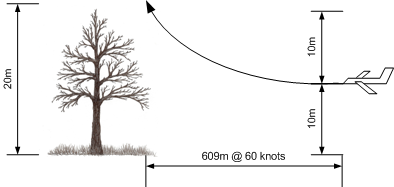
\includegraphics[width=300pt,height=160pt]{./Figures/ProblemStatement.png}
\caption {Case study for obstacle detection requirement}
\label{ob}
\end{figure}

Although digital terrain map are generally available for flight path 
planning and in flight navigation, it does not have the resolution to 
indicate all hazardous obstacle such as tall trees, steep hills, or 
man-made tall objects. The obstacle detection and avoidance system must 
be in place to detect discrete threat, and operate automatically with 
minimum intervene from the operator. 

\section{Contributions}\label{section:Contribution}
The thesis reviews the properties and consistency of a typical Extended 
Kalman Filter (EKF) based SLAM algorithm, and discusses the advantage 
and limitation of vision based SLAM method. The analysis motivates the 
development of an improved method by fusing multiple sensors into a mono 
vision EKF based SLAM framework.

Using a monocular vision for mapping is a bearing only SLAM problem. The 
measurement is through projection, which loses information about the 
relative position of the feature since the range is unknown. Without 
camera motion measurements, map created by monocular vision can be 
scaled arbitrarily. For a SLAM application in aerial scenario, camera 
vibration and sudden movement is common when aircraft is hit by cross 
wind, which can cause the lost of tracked features. A recursive EKF 
based SLAM algorithm is described in this thesis. The method utilizes 
sensor onboard the UAV to provide motion measurement of the camera, and 
improve the robustness of the algorithm under rough flying condition. 
Real aerial data were collected to test the performance and accuracy of 
the algorithm in a scenario similar to the one where the UAV will be 
eventually deployed. The preliminary result of the test flight was 
published in []. This paper is one of the first ones in the field 
that successfully applying monocular vision SLAM in large scale aerial 
application. A more thorough analysis on the behavior of the algorithm 
and its error is presented in this thesis.Furthermore, a number of 
baseline separations for the cameraare tested to optimize the 
performance and computation cost of the algorithm. 

\section{Organization}\label{section:Organization}
The thesis is organized as follows:

\begin{itemize}
\item Chapter 2 presents an overview on sensors, computer vision 
algorithms, SLAM algorithm related to obstacle detection and range 
measurement.
\item Chapter 3 describes the detail implementation of the proposed 
multisensory monocular SLAM algorithm.
\item Chapter 4 describes camera calibration procedure, equipments setup 
for the aerial data collection, and data preparation steps. 
\item Chapter 5 presents detail analysis on the performance of the 
algorithm. Convergence and consistency of the algorithm is discussed in 
section and . Error analysis compared to ground truth data is presented 
in and . The effect of using multiple sensors in improving the 
robustness is discussed in . At last, the camera baseline optimization 
is given in .
\end{itemize}

%%% Local Variables:
%%% mode: latex
%%% TeX-master: "thesis.tex"
%%% End:
